\documentclass[T,J]{fose} % 「コンピュータソフトウェア」用のクラスファイルは compsoft です.
\taikai{2023} % 固定です.出版委員長が毎年変更してAuthor Kitを配布してください.

\usepackage [dvipdfmx] {graphicx}

% ユーザが定義したマクロなどはここに置く.ただし学会誌のスタイルの
% 再定義は原則として避けること.

\usepackage[dvipdfmx]{graphicx}
\usepackage[dvipdfmx]{color}
\usepackage{comment}
\usepackage{booktabs}
\usepackage{color}
\usepackage{latexsym}
\usepackage{paralist}
\usepackage{listings, jvlisting}
\usepackage{url}
\usepackage{balance}
\usepackage{multirow}
\usepackage{amsmath}
\usepackage{fancybox}
\usepackage{ascmac}
\usepackage{listings}
\usepackage{tabularx}
\usepackage{xurl}
\usepackage{cite}
\usepackage{subcaption}
\usepackage{url}
\usepackage{otf}

% 以下のマクロはサンプルファイル作成用のマクロです.不要であれば削除してください.

\begin{document}

% 論文のタイトル
\title{GitHub Copilotを用いたコード推薦における\\入力言語の影響調査}
\setetitle{Investigation of the effect of input languages on code recommendation using GitHub Copilot}
\author{小\UTF{6801} 慶 野口 広太郎 王 棟 近藤 将成 亀井 靖高 鵜林 尚靖
%
% ここにタイトル英訳 (英文の場合は和訳) を書く.
% 英語タイトルは論文1ページ目左下,著者らの名前・所属一覧の一番上に表示される
%
% 上記\setetitle中で改行した場合は "\etitle" を削除し,改行(\\)を入れていないタイトルを記載してください.
% \ejtitleは1ページ目左下に挿入されるタイトルとして使用されます.
% また,"\etitle"はFOSE論文フォーマット独自のマクロです.
\ejtitle{\etitle}
%
% ここに著者英文表記 および
% 所属 (和文および英文) を書く.
% 複数著者の所属はまとめてよい.
%
\shozoku{Kei Koyanagi}{九州大学}
{Kyushu University}
% 複数著者の所属は以下のようにまとめてよい.
\shozoku{Kotaro Noguchi, Dong Wang, Masanari Kondo, Yasutaka Kamei, Naoyasu Ubayashi}{九州大学}
{Kyushu University}
}

%
% 和文アブストラクト
% In English paper, content of Jabstract will be ignored. 
\Jabstract{
  近年,IT需要の拡大に伴って,開発効率向上のため,開発支援ツールを活用して開発が行われている.
  その中の一つとして,2022年にGitHubが公開したGitHub Copilotがある.
  GitHub Copilotは大規模言語モデルをベースとしたコード推薦ツールの一種であり,
  仕様を記述したコメントや,記述中のプログラムをもとに開発者に対してコードやライブラリを推薦する.
  一方,大規模な事前学習済み言語モデルは,入力によって出力が大きく異なることが知られている.
  そこで,本稿では,言語間のニュアンスの違いに着目し,入力言語の違いがCopilotの性能にどのような影響を与えるのか調査を行った.
  調査の結果,入力言語の違いによってGitHub Copilotの性能に差が生じることが明らかになった.
  また,調査結果によって明らかとなった大規模言語モデルに対する問題点を示す.
}
%
% 英文アブストラクト(本サンプルの原論文にはなし)
%\Eabstract{
%I will write English abstract here after the review of Japanese abstract.
%}
%
\maketitle \thispagestyle {empty}
{
\section{はじめに\label{intro}}
    近年,IT需要の拡大に伴って,開発効率の向上のためにタスク管理ツールやプロジェクト管理ツールをはじめ,様々な支援ツールを活用して開発が行われている.
    その中の一つとして,2022年にGitHubが公開したGitHub Copilotがある(以下,Copilotと記述する).
    Copilotは大規模言語モデルをベースとしたコード推薦ツールの一種であり,使用を記述したコメントや,記述中のプログラムをもとに開発者に対してコードやライブラリを推薦する.
    そのため,フルスクラッチする必要がなく,開発コストの削減が見込まれる.

    一方,大規模な事前学習済み言語モデルは,入力によって出力が大きく異なることが知られている.
    そのため,言語モデルの能力を最大限引き出すためには,適切なコメントを入力する必要がある.
    
    また,現在世界では7000語以上の言語が存在すると言われているが,言語によって使用頻度は異なる.
    そのため,コメントに異なる言語を使用することで,学習データ数の不均衡などにより学習結果のバイアスにつながる可能性があると考えた.
    そこで本研究では,言語間のニュアンスの違いに着目し,言語の違いがCopilotの性能にどのような影響を与えるのか調査を行った.

    以降,第2章で関連研究および本研究の目的,
    第3章で本研究の実験設計について述べる.
    第4章で調査結果を示し,第5章で考察を行う.
    第6章では,妥当性の脅威を説明し,
    最後に第7章で結論と今後の課題について述べる.

\section{背景と目的\label{related_research}}

\subsection{本研究の目的}
  急速に進むIT化に伴い,事前学習済み大規模言語モデルの活用が進んでおり,
  今後ますます大規模言語モデルが組み込まれたシステムが拡大していくことが予想される.
  その中の一つであるCopilotに対しても研究が盛んに行われている\cite{Yao2022ACL}\cite{Nguyen2022MSR}\cite{Sobania2022GECCO}\cite{Dakhel2022arXiv}\cite{Vaithilingam2022CHI}.
  一方で,大規模な事前学習済み言語モデルは,
  入力によって出力が大きく異なることが知られている\cite{Yao2022ACL}.
  そのため,言語モデルの能力を最大限引き出すためには,適切なコメントを入力する必要がある.
  コメントは主要な要素として入力言語と入力内容で構成されるが,
  入力言語の違いによる性能への影響については調査が行われていない.
  そこで,入力言語の違いによる性能への影響を調査することで,
  システムの性能を最大限引き出すための手がかりを得ることができると考えた.
  本稿では,日本語,英語,および中国語の3言語を入力とした場合のそれぞれのCopilotの性能を比較する.
  調査課題を以下に示す.

  
  \begin{itemize}
    \item[\textbf{RQ}] \textbf{入力する言語の違いによって,Copilotの性能にどのような影響を与えるのか}
      \item[目的]{
      現状,大規模な事前学習済み言語モデルは,入力によって出力が大きく異なり,
      主な要素として,入力内容および入力言語がある.
      本研究では,後者の言語に着目し,入力言語によってCopilotの性能に差が生じるのか明らかにすることで,
      今後のCopilotの最適な活用についての知見を得る.}
  \end{itemize}

\subsection{関連研究}
  コード生成におけるプロントエンジニアリングとは,モデルに対してどのようなプロンプトを入力として与えれば生成精度がより向上するかを探索する手法である.
  プロンプトとはモデルに対して与える入力のことで,モデルに対して与える入力としてはコードの仕様やプログラムそのものなどがある.
  モデルは与えられたプロンプトをもとに,次にどのようなをコードを生成するかを予測する.
  
  Yaoら\cite{Yao2022ACL}は,プロンプトとして入力するサンプルの入力順序の違いによって,GPT-3のような
  大規模な事前学習済み言語モデルの性能にどのような影響を与えるのか調査を行った.
  その結果,サンプルの入力順序によって性能にばらつきが生じ,
  これがモデルサイズに関係なく発生すること,サンプルの特定のセットに関係なく発生すること,
  およびあるモデルには優れた学習順序であっても別のモデルには適用できないことを示した.
  
  \noindent また,各モデルに対して優れた性能を示すプロンプトの探索手法としてエントロピーベースでの探索手法を提案した.
  このエントロピーベースの手法では,Global Entropy(以下GlobalE)とLocal Entropy(以下LocalE)が用いられている.
  GlobalEは各入力に対して極端にアンバランスな予測を避けるプロンプトを特定するため,
  LocalEは学習データに対して過度に高性能な予測を避けるプロンプトを特定するために使用されている.
  調査の結果,エントロピーベースでの探索手法は,ランダムにプロンプトを選択するよりも優れた性能を示した.

  Nguyen\cite{Nguyen2022MSR}らは,Copilotのコード推薦の精度および推薦されたコードの品質について,
  異なるプログラミング言語で調査を行った.
  LeetCodeの問題に対してEasy, Medium, Hardの3つの難易度で調査を行ったところ,
  Easyでは全てのプログラミング言語が全テストケースを通過し,全体として,Java, Python, C, Javascriptの順に高い精度を示した.
  また,推薦されたコードの品質については,プログラミング言語間における差はほとんど生じず,
  判読性は高いことを示した.


  
\section{実験設計\label{approach}}
  本章では,本研究で行った実験の概要について説明する.
  \begin{figure}[t]
    \centering
    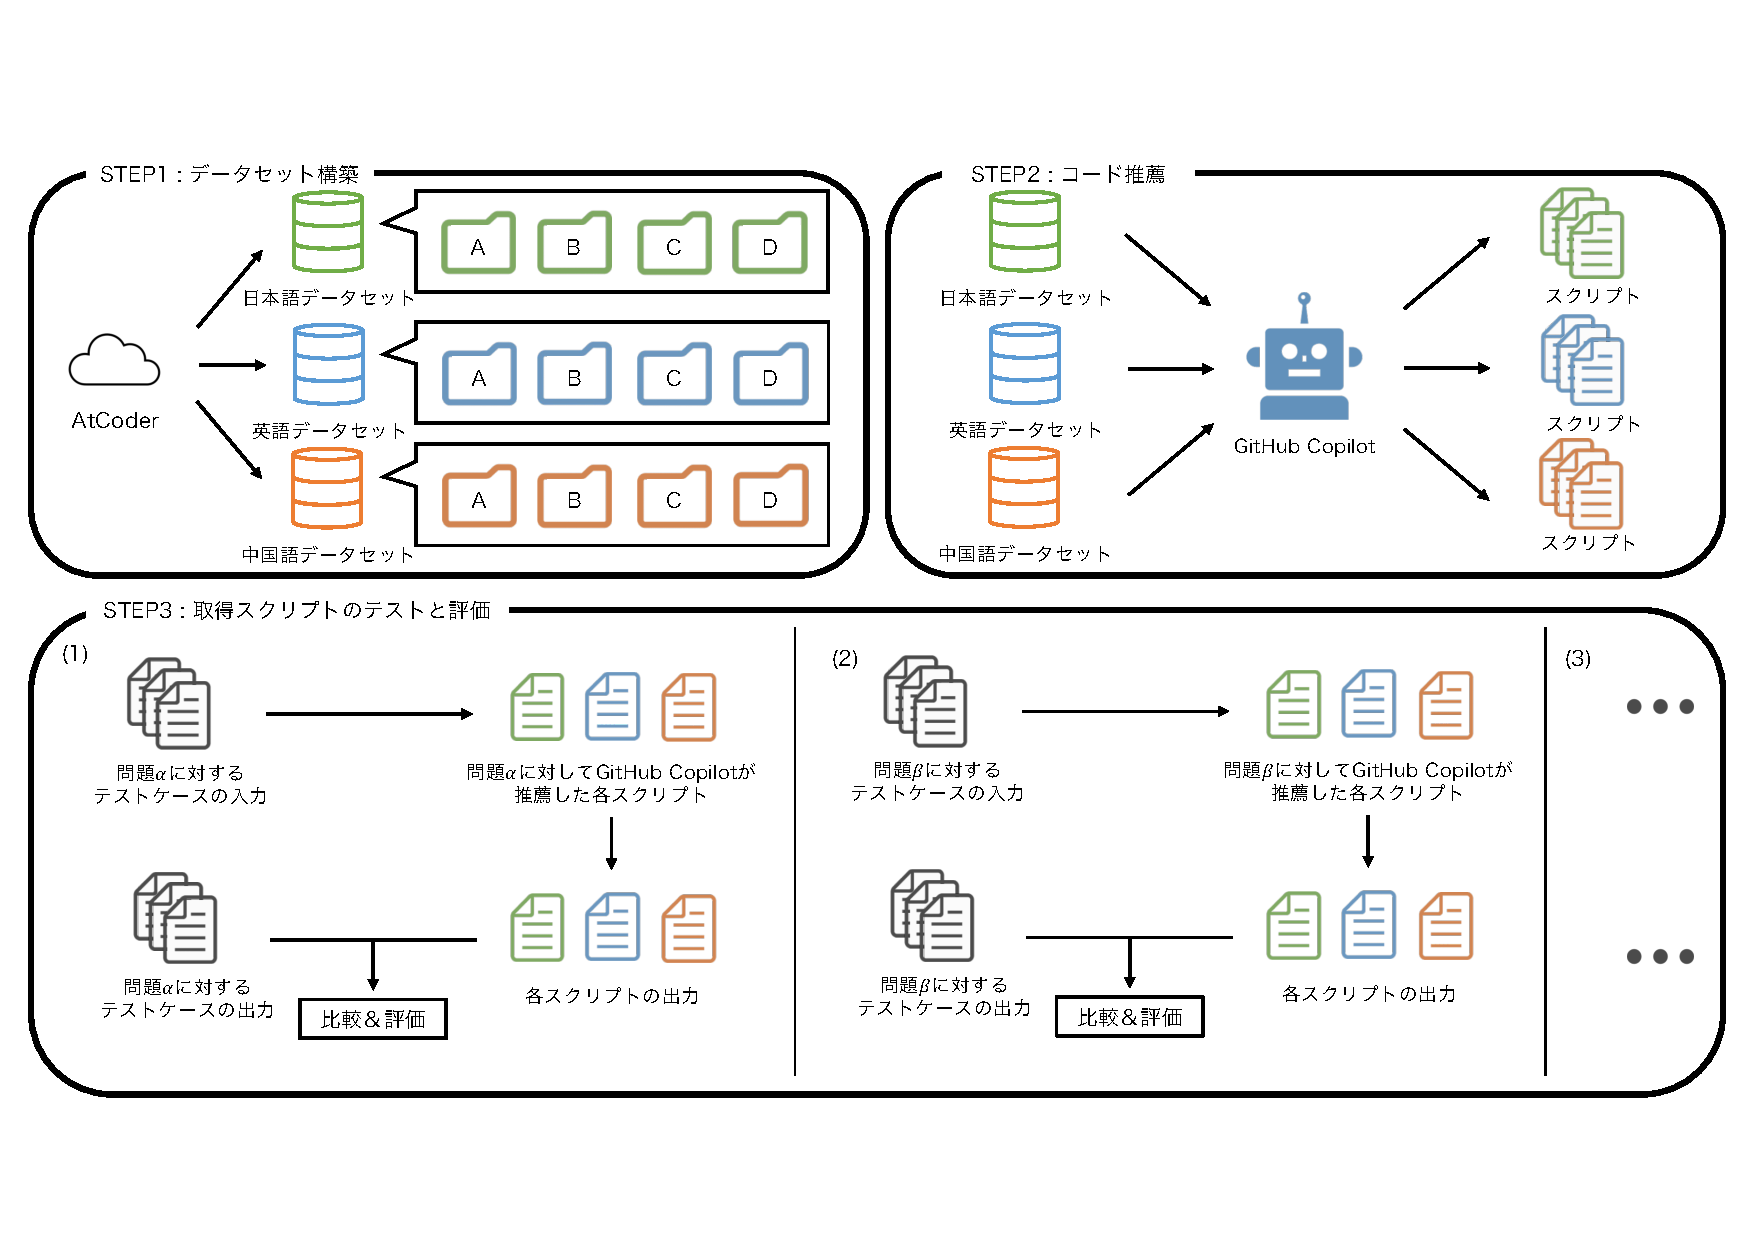
\includegraphics[width=\linewidth]{image/system.pdf}
    \caption{実験設計の概要}
    \label{experiment_design}
  \end{figure}
  
  \subsection{データセット構築\label{build_dataset}}
    本研究では日本国内において最大の競技プログラミングコンテストであるAtCoder\cite{AtCoder}の問題を使用する.
    中でも,AtCoder Beginner Contestという毎週開催されているコンテストの問題を使用する.
    このコンテストは6/24までに1${\sim}$307(2023/06/24現在)の問題が公開されており,
    各問題の難易度はA, B, C, D, E, F, G, Ex(H)までの最大8段階でアルファベットの語順が後になるほど難易度が高くなる.
    また,問題は日本語版と英語版が準備されている.
    この問題から,問題番号99${\sim}$287,各問題の難易度A${\sim}$Dの日本語版および英語版を使用する.
    問題を限定する理由としては,
    問題番号は十分なテストケースの数が確保されている問題を使用するため,
    問題難易度は事前実験にてCopilotが正しいプログラムを生成できる境目であったためである.
    続いて,中国語版の問題はAtCoderには存在しないため,
    英語版のデータセットをDeepL APIを使用して翻訳し,
    翻訳した問題をネイティブによる校正を行うことで,中国語版のデータセットを作成した.
    最終的に,問題番号が99${\sim}$287,各問題の難易度がA,B,C,D,問題の言語が英語,日本語,中国語の三つのデータセットが取得でき,
    これらを本実験のデータセットとした.

  \subsection{プログラム推薦\label{recommend_program}}
    \ref{build_dataset}節で作成したデータセットに対して,Copilotでプログラム推薦を行う.
    \ref{build_dataset}節で作成した各言語のデータセットの中には,問題番号が99${\sim}$287,各問題の難易度がA,B,C,D存在するため,合計で2,268問存在する.
    これらの問題に対して,プログラム推薦を行う.
    
    \begin{table}[t]
      \caption{問題102-Aの英語版}
      \begin{tabular}{c}
        \begin{tabularx}{23zw}{X}
          \hline
          \verb|#Problem Statement| \\
          \verb|#You are given a positive integer N.| \\
          \verb|#Find the minimum positive integer | \\
          \verb|#divisible by both 2 and N.| \\
          \verb|#Constraints| \\
          \verb|#1 ≦ N ≦ 10^9| \\
          \verb|#All values in input are integers.| \\
          \verb|#Input| \\
          \verb|#Input is given from Standard Input | \\
          \verb|#in the following format:| \\
          \verb|#N| \\
          \verb|#Output| \\
          \verb|#Print the minimum positive integer | \\
          \verb|#divisible by both 2 and N.| \\
          \verb|#Sample Input 1| \\
          \verb|#3| \\
          \verb|#Sample Output 1| \\
          \verb|#6| \\
          \hline
        \end{tabularx}
      \end{tabular}
      \label{problem_102_A_en}
    \end{table}

    表\ref{problem_102_A_en}は問題102-Aの英語版のデータセットの中身である.
    このように各問題のデータセットには,問題,制約,入力,出力,サンプル入力,サンプル出力がコメントとして記述されている.
    ただし,問題によってサンプル入力およびサンプル出力の数は異なり,また注釈等の記述がある場合もある.
    このデータセットを入力として,Copilotによるプログラム推薦を行い,$x$個の推薦プログラムを得る.
    このとき,$x$は$0 {\leq} x {\leq} 10$を満たす.
    また,推薦プログラムで出力するプログラミング言語はPythonを使用した.
    この入力から出力までの流れを各問題に対して5回実行する.
    その理由としては,Copilotの推薦スクリプトが毎回変化するため,
    このランダム性を考慮して,評価を行うためである.
    
  \subsection{取得プログラムのテストと評価\label{test_and_evaluation}}
    \ref{recommend_program}節で取得したプログラムに対して,テストを行う.
    このテストは,各問題に対して,テストケースの入力を入力として取得したプログラムを実行し,テストケースの出力と一致するかを確認する.
    そして,各推薦スクリプトが全てのテストケースを通過したか否かで評価を行う.
    使用した評価指標は,$Accuracy$(正答率)で,推薦された全スクリプトの内,全てのテストケースを通過したスクリプトの割合を示す.



\section{結果\label{result}}
  \begin{table}[t]
    \centering
    \caption{英語における$Accuracy$}
    \label{En_accuracy}
    \scalebox{0.6}{
    \begin{tabular}{|c|c|c|c|c|c|c|c|c|}
      \hline
      %推薦 & \multicolumn{2}{c|}{} & \multicolumn{2}{c|}{} & \multicolumn{2}{c|}{} & \multicolumn{2}{c|}{} \\
      {推薦} & \multicolumn{2}{c|}{A} & \multicolumn{2}{c|}{B} & \multicolumn{2}{c|}{C} & \multicolumn{2}{c|}{D} \\
      \hline
      1st & 63.7 & 864/1357 & 51.0 & 860/1686 & 28.3 & 482/1702 & 10.4 & 172/1657 \\
      \hline
      2nd & 65.4 & 878/1343 & 50.5 & 858/1698 & 26.7 & 471/1761 & 10.0 & 182/1813 \\
      \hline
      3rd & 63.6 & 856/1346 & 50.9 & 811/1594 & 26.6 & 438/1648 & 9.31 & 151/1622 \\
      \hline
      4th & 60.4 & 819/1355 & 51.6 & 842/1631 & 31.3 & 499/1596 & 11.0 & 167/1524 \\
      \hline
      5th & 60.4 & 831/1375 & 50.5 & 857/1698 & 31.1 & 552/1774 & 12.0 & 217/1812 \\
      \hline
      \end{tabular}
    }
  \end{table}

  \begin{table}[t]
    \centering
    \caption{日本語における$Accuracy$}
    \label{Ja_accuracy}
    \scalebox{0.6}{
    \begin{tabular}{|c|c|c|c|c|c|c|c|c|}
      \hline
      {推薦} & \multicolumn{2}{c|}{A} & \multicolumn{2}{c|}{B} & \multicolumn{2}{c|}{C} & \multicolumn{2}{c|}{D} \\
      \hline
      1st & 68.7 & 857/1248 & 52.8 & 872/1651 & 28.9 & 482/1668 & 10.0 & 170/1697 \\
      \hline
      2nd & 67.4 & 840/1246 & 52.9 & 824/1559 & 28.4 & 454/1597 & 10.2 & 155/1526 \\
      \hline
      3rd & 68.1 & 842/1237 & 54.3 & 879/1619 & 28.5 & 449/1577 & 11.0 & 153/1391 \\
      \hline
      4th & 68.4 & 860/1258 & 57.6 & 872/1515 & 33.1 & 439/1328 & 12.8 & 125/974 \\
      \hline
      5th & 68.0 & 849/1249 & 54.5 & 922/1693 & 32.7 & 592/1813 & 11.4 & 208/1832 \\
      \hline
      \end{tabular}
    }
  \end{table}
  
  \begin{table}[t]
    \centering
    \caption{中国語における$Accuracy$}
    \label{Zh_accuracy}
    \scalebox{0.6}{
    \begin{tabular}{|c|c|c|c|c|c|c|c|c|}
      \hline
      {推薦} & \multicolumn{2}{c|}{A} & \multicolumn{2}{c|}{B} & \multicolumn{2}{c|}{C} & \multicolumn{2}{c|}{D} \\
      \hline
      1st & 52.7 & 739/1402 & 40.1 & 705/1757 & 22.7 & 405/1787 & 7.70 & 136/1766 \\
      \hline
      2nd & 52.5 & 728/1386 & 43.1 & 734/1703 & 21.9 & 376/1718 & 7.81 & 134/1715 \\
      \hline
      3rd & 52.1 & 737/1415 & 39.7 & 687/1730 & 22.7 & 405/1788 & 8.11 & 143/1764 \\
      \hline
      4th & 51.8 & 732/1412 & 41.5 & 717/1728 & 23.2 & 413/1783 & 8.35 & 146/1748 \\
      \hline
      5th & 51.5 & 739/1436 & 41.9 & 728/1738 & 22.0 & 395/1798 & 7.57 & 132/1744 \\
      \hline
      \end{tabular}
    }
  \end{table}

  \begin{table}[t]
    \centering
    \caption{各言語の$Accuracy$の中央値}
    \label{Med_accuracy}
    \scalebox{0.9}{
    \begin{tabular}{|c|c|c|c|c|}
      \hline
      {} & A & B & C & D \\
      \hline
      英語 & 63.6\% & 50.9\% & 28.3\% & 10.4\% \\
      \hline
      日本語 & 68.1\% & 54.3\% & 28.9\% & 11.0\% \\
      \hline
      中国語 & 52.1\% & 41.5\% & 22.7\% & 7.81\% \\
      \hline
      \end{tabular}
    }
  \end{table}

  本章では,RQと結果,および本実験で得られた結果に対する追加実験の必要性を示す.
  なお,本実験は2023/4${\sim}$2023/7に実施した.
  %\begin{description}
    %\item[\noindent\textbf{RQ:入力する言語の違いによって,Copilotの性能にどのような影響を与えるのか}]
  %\end{description}

  \subsection{RQへの回答}
  \noindent\textbf{RQ:入力する言語の違いによって,Copilotの性能にどのような影響を与えるのか}

  \noindent\textbf{結果:}表\ref{En_accuracy},表\ref{Ja_accuracy},および表\ref{Zh_accuracy}は
  それぞれ英語,日本語,および中国語における$Accuracy$を示したものである.
  表の各行は,各推薦で得られた総推薦コード数と全てのテストケースを通過した推薦コード数を表している.
  これらの表から,生成毎に$Accuracy$にばらつきが生じているため,Copilotが毎回異なるコードを推薦していることがわかる.
  また,推薦回数を重ねるほど$Accuracy$の値が単調に増加したり,減少したりすることはなかった.\par
  
  表\ref{En_accuracy}より,英語のデータセットにおいて,A問題では最大5.0\%,B問題では最大1.1\%,C問題では最大4.7\%,D問題では最大2.7\%の差が生じた.
  また,表\ref{Ja_accuracy}より,日本語のデータセットにおいて,A問題では最大1.3\%,B問題では最大4.8\%,C問題では最大4.7\%,D問題では最大2.8\%,
  表\ref{Zh_accuracy}より,中国語のデータセットにおいては,A問題で最大1.2\%,B問題で最大3.4\%,C問題で最大1.3\%,D問題で最大0.78\%の差が生じた.

  また,言語別で推薦された全コード数を平均すると,英語のデータセットでは,A問題が1355個,B問題が1661個,C問題が1696個,D問題が1686個,
  日本語のデータセットでは,A問題が1247個,B問題が1607個,C問題が1596個,D問題が1484個,
  中国語のデータセットでは,A問題が1410個,B問題が1731個,C問題が1774個,D問題が1747個であった.
  これらの結果から,日本語のデータセットでは,英語のデータセットと中国語のデータセットに比べて,推薦された全コード数が少なかった.
  加えて,全難易度で日本語のデータセットの$Accuracy$が最も高かった.
  %これは,日本語での入力により,Copilotがより最適なスクリプトのみを推薦していることを示している.
  %この理由として,AtCoder\cite{AtCoder}が日本で運営されているため,
  %より多くの日本人がAtCoderを使用しており,日本語のコメントを含んだ回答がGitHub上にアップロードされ,それらが学習時に多く使用されたためであると考えられる.      
  さらに,表\ref{Med_accuracy}は,各言語の難易度別の$Accuracy$の中央値を示したものである.   
  表\ref{Med_accuracy}より,中国語のデータセットは,英語のデータセットに比べて,日本語のデータセットとの$Accuracy$の差が大きかった.
  %これは,AtCoder\cite{AtCoder}において,日本語と英語の問題が準備されているため,
  %日本語や英語のコメントを含んだより多くの正解プログラムが学習時に使用されたためであると考えられる.
  %さらに中国語の生成スクリプトが最も多かった原因としては,
  %AtCoderの中国語版が存在しないため,GitHub上に中国語のコメントを含んだ正解プログラムが少なく,
  %推薦プログラムが絞りきれず,多くのスクリプトが推薦された可能性がある.

  \begin{screen}
    GitHub Copilotの推薦コードの正答率は,入力言語によって変化し,
    日本語,英語,中国語の順に$Accuraccy$が高かった.
  \end{screen}

  \subsection{追加実験の必要性\label{future_work}}
    本研究では,AtCoder\cite{AtCoder}の開催番号99${\sim}$287,
    各問題の難易度A, B, C, D,各問題の言語を日本語,英語,中国語を対象として調査を行った.
    その結果,日本語を用いてコード中にコメントを入力する場合の方が,
    英語や中国語を用いてコメントを入力する場合よりも,正答率が高いことがわかった.
    現在の世の中において,世界で最も使用されている言語は英語である\cite{Ethnologue}ため,
    入力に使用する言語が英語である場合の方が,正答率が高いことが経験的に知られている.
    しかし今回の結果より,ある特定のタスクにおいては英語以外の言語を使用した方が正答率が高い可能性が示唆された.
    ただし,本研究では特定のデータセットに対して調査を行ったため,
    調査結果をより一般化する必要がある.
    そこで,英語圏で行われているプログラミングコンテストの問題を日本語および中国語に翻訳,
    また中国語圏で行われているプログラミングコンテストの問題を英語および日本語に翻訳した
    データセットを使用して今後調査を行う所存である.


  
  \vskip\baselineskip

\section{考察\label{discussion}}
  \begin{figure}[t]
    \begin{verbatim}
      =======
      Suggestion 1

      def alloy(a,b):
          if a == 0:
              return 'Silver'
          elif b == 0:
              return 'Gold'
          else:
              return 'Alloy'
    \end{verbatim}
    \caption{問題212-Aの中国版に対する推薦コードの一例}
    \label{recommend_212_A_en}
  \end{figure}
  \ref{result}章で示した結果について,現時点での筆者の考察を述べる.
  これらは筆者の考察であるため,今後の実験により検証されなければならない.
  \subsection{推薦コードの生成数と正答率の関係}
  表\ref{En_accuracy}, \ref{Ja_accuracy}, \ref{Zh_accuracy}のうち,
  各言語の$Accuracy$の差が3.0\%以上だった問題の最大値に着目すると,推薦された全コード数が5回のうち最も少なく,
  このことから,推薦1回につき推薦コードを最大10個取得することで,かえって$Accuracy$が低下した可能性が考えられる.

  また,難易度別に推薦された全コード数に着目すると,A問題はB, C, D問題に比べて,推薦された全コード数が最も少なかった.
  これはA問題が基本的な文法を問う問題であるため,処理が単純であり,
  類似した文面のコードが推薦されると重複として除外されている可能性があると考えた.

  さらに,言語別で推薦された全コード数の平均と日本語のデータセットの$Accuracy$が最も高かったことより,
  日本語での入力により,Copilotがより最適なコードのみを推薦していることがわかる.
  これは,AtCoder\cite{AtCoder}が日本で運営されているため,
  多くの日本人がAtCoderを使用しており,日本語のコメントを含んだ回答がよりアップロードされ,それらが学習時に多く使用されたためであると考えられる.
  \subsection{中国語データセットにおける正答率の低下}
  表\ref{Med_accuracy}より,中国語のデータセットは,英語のデータセットに比べて,日本語のデータセットとの$Accuracy$の差が大きかった.
  これは,AtCoder\cite{AtCoder}において,日本語と英語の問題が準備されているため,
  日本語や英語のコメントを含んだより多くの正解コードが学習時に使用されたためであると考えられる.
  さらに中国語の生成コードが最も多かった原因としては,
  AtCoderの中国語版が存在しないため,中国語のコメントを含んだ正解コードの数が少なかった可能性がある.
  これに対して中国語を基とするプログラミングコンテストのデータセットを使用して調査を行う必要がある.
  
  また,A問題に関しては特に大きな差が生じ,日本語との差が16.0\%,英語との差が11.5\%であった.
  A問題は今回使用したデータセットの難易度の中で最も簡単な問題であるため,
  $Accuracy$の値に大きな差が生じにくいと予測していたが,予測とは異なる結果となった.
  その理由として,AtCoder\cite{AtCoder}において,日本語と英語の問題が準備されているため,
  簡単な問題であっても,これらの言語をコメントに含んだより多くの正解コードがアップロードされており,
  それらが学習に使用された可能性がある.

  その他の原因探索のため,実際に$Accuracy$の差が大きかった問題をいくつか確認した.
  図\ref{problem_212_A_en}の問題は,
  英語および日本語のデータセットでは,全ての推薦コードが全てのテストケースを通過しているが,
  中国語のデータセットでは,全ての推薦コードが全てのテストケースを通過していない例である.
  また,図\ref{recommend_212_A_en}は実際に問題212-Aにおける中国語のデータセットに対する推薦コードである.
  図\ref{recommend_212_A_en}のような,単純な条件のみで構成されているものや,
  条件分岐の途中で推薦が打ち切られているもの,条件分岐の数が少ないものであった.
  
  この問題のように,条件が複数ある場合や,条件が複雑である場合,出力が文字列である場合に
  特に英語および日本語との$Accuracy$の差が大きくなる傾向があった.
  この原因として,AtCoderの文字列の出力形式がローマ字や英単語であるため,
  入力として使用した中国語のデータセットの文章中にローマ字や英単語が含まれており,
  それらがシンボルとして認識されなかった可能性や翻訳してデータセットを作成した影響が考えられる.
\section{妥当性への脅威\label{threats}}

\noindent{\textbf{内的妥当性.}}
  本研究では,各プロジェクトの
  `requirements.txt'からライブラリ使用情報を取得して調査を行った.
  ただしファイル名は任意に設定可能なため,
  別のファイル名を使用している,
  あるいは,`requiments.txt'ファイルを設定していない場合がある.
  そのため,対象にすべきファイルを取得できていない可能性を考慮し,
  実際のプログラムからも情報を抽出して実験を行う必要がある.

\noindent{\textbf{外的妥当性.}}
  本研究では,Pythonの機械学習ライブラリの使用率上位12件%\cite{Kaggle}
  のライブラリを最低1つ使用している
  プロジェクトのうち,GitHubでのスター数各上位100件までを対象に調査を行ったが,
  調査結果をより一般化するためには,
  依存ライブラリ数,および対象のプロジェクト数を増加させて調査を行う必要がある.


\section{おわりに\label{conclusion}}
  本稿では日本語,英語,中国語のデータセットを使用して,
  GitHub Copilotによるプログラム推薦を行い,その正答率を比較した.
  調査の結果,日本語,英語,中国語の順に正答率が高く,
  英語と中国語にはA問題において約11.5\%の差が生じた.
  今後の課題として,データセットを変更した調査,
  およびコードの品質を評価する調査が必要である.
  

}

\textbf{謝辞}

本研究の一部は JSPS 科研費JP20H04167,JP21H04877,JP22K17874,JP22K18630の助成を受けた.


\bibliographystyle{jssst}
\bibliography{references}

\end{document}

